\documentclass[60pt]{article}
\usepackage[a4paper, margin={1in, 1in}]{geometry}
\usepackage[utf8]{inputenc}
\usepackage{polski}
\usepackage{mathtools}
\usepackage{amsfonts}
\usepackage{amssymb}
\usepackage{amsmath}
\usepackage{multicol}
\usepackage{paralist}
\usepackage{tabto}
\usepackage{graphicx}
\usepackage{etoolbox}
\usepackage{changepage}
\usepackage{tasks}
\usepackage{pgfplots}
\usepackage{fancyhdr}
\usepackage{mathtools}
\usepackage{tikz}
\DeclarePairedDelimiter\ceil{\lceil}{\rceil}
\DeclarePairedDelimiter\floor{\lfloor}{\rfloor}
\usepackage{graphicx}

\usepackage{minted}
\usemintedstyle{autumn}

\DeclareMathOperator{\arctg}{arctg}
\DeclareMathOperator{\sh}{sh}
\DeclareMathOperator{\ch}{ch}
\DeclareMathOperator{\sgn}{sgn}

\let\arctan\relax
\DeclareMathOperator{\arctan}{arctg}
\let\tan\relax
\DeclareMathOperator{\tan}{tg}

\pagestyle{fancy}

%Ściana tekstu

%Ściana tekstu

\title{Pojekt szkolnej bazy danych}
\author{Jakub Kołodziejczyk, Konrad Nowak, Wojciech Węgrzyn}


\begin{document}
\maketitle

\newpage
\tableofcontents

\newpage
\section{Wstęp}

\subsection{Cel projektu}

Nasza grupa obrała sobie za cel utworzenia bazy danych szkoły. Sugerowaliśmy się raczej działaniem szkół na poziomie licealnym, stąd też w naszej bazie danych pojawiają się koła naukowe, przedmioty fakultatywne czy stypendia. 

\subsection{Główne założenia}

Głównym założeniem naszej grupy było utworzenie bazy danych, która pozwalałaby organom zarządzającym na łatwą analizę dziejów szkolnych. 

Nasz projekt nie pretenduje do bycia zastępnikiem elektronicznego dziennika typu Librus czy Synerga. Staraliśmy się raczej stworzyć bazę, która będzie dawała przejrzyste informacje zarządzania organizacją szkoły, stąd też wprowadziliśmy specjalne tabele typu urlopy, dni wolne czy usprawiedliwienia. 

Głównymi ograniczeniami naszej bazy są dwa fakty:

Pierwszy z nich to limit przedmiotów, których może uczyć dany nauczyciel. Nasz projekt pozwala jednemu nauczycielowi prowadzić jeden zwykły przedmiot oraz jeden fakultatywny. Mamy świadomość alternatywnych rozwiązań tego problemu, ale postanowiliśmy zdecydować się na taką implementację ze względu na możliwości analizy danych, na które pozwala obecny stan rzeczy. 

Drugim problemem naszego projektu, który mógłby nie sprostać oczekiwaniom potencjalnego klienta jest uproszczony system rejestracji ocen uczniów. Jak wcześniej wspomnieliśmy, nie zamierzaliśmy utworzyć dziennika elektronicznego, a raczej system pozwalający na analizę danych - możemy sprawdzić ile ocen ma dany uczeń, jaką ma średnią, ile ocen wystawił dany nauczyciel i inne odpowiednimi procedurami. Niemniej nie implementujemy wagi ocen czy też ocen rocznych z całych przedmiotów, ponieważ nie to było naszym celem.

\subsection{Możliwości}

\subsection{Ograniczenia przyjęte przy projektowaniu}

Nasza baza danych obsługuje jedynie oceny w postaci typu danych INT, stąd też nie są możliwe oceny cząstkowe. 

\subsection{Strategia pielęgnacji}

Głównym założeniem pielęgnacji naszej bazy danych byłaby comiesięczna pełna kopia zapasowa oraz różnicowa kopia danych tydzień. 

Ze względu na potencjalną niewielką dynamikę naszej bazy taka częstotliwość backupów powinna być wystarczająca. 

Najbardziej dynamiczną naszą tabelą będzie tabela "Oceny" - pomijając ją oraz tabelę "Usprawiedliwienia" nie oczekujemy regularnych i częstych zmian w naszej bazie. Zdecydowana ich większość jest raczej statyczna, określana najczęściej co semestr, a w niektórych wypadkach nieregularnie, lecz nieco częściej (na przykład "Urlopy").

\newpage
\section{Schematy}

\subsection{Diagram ER}

\begin{figure}
  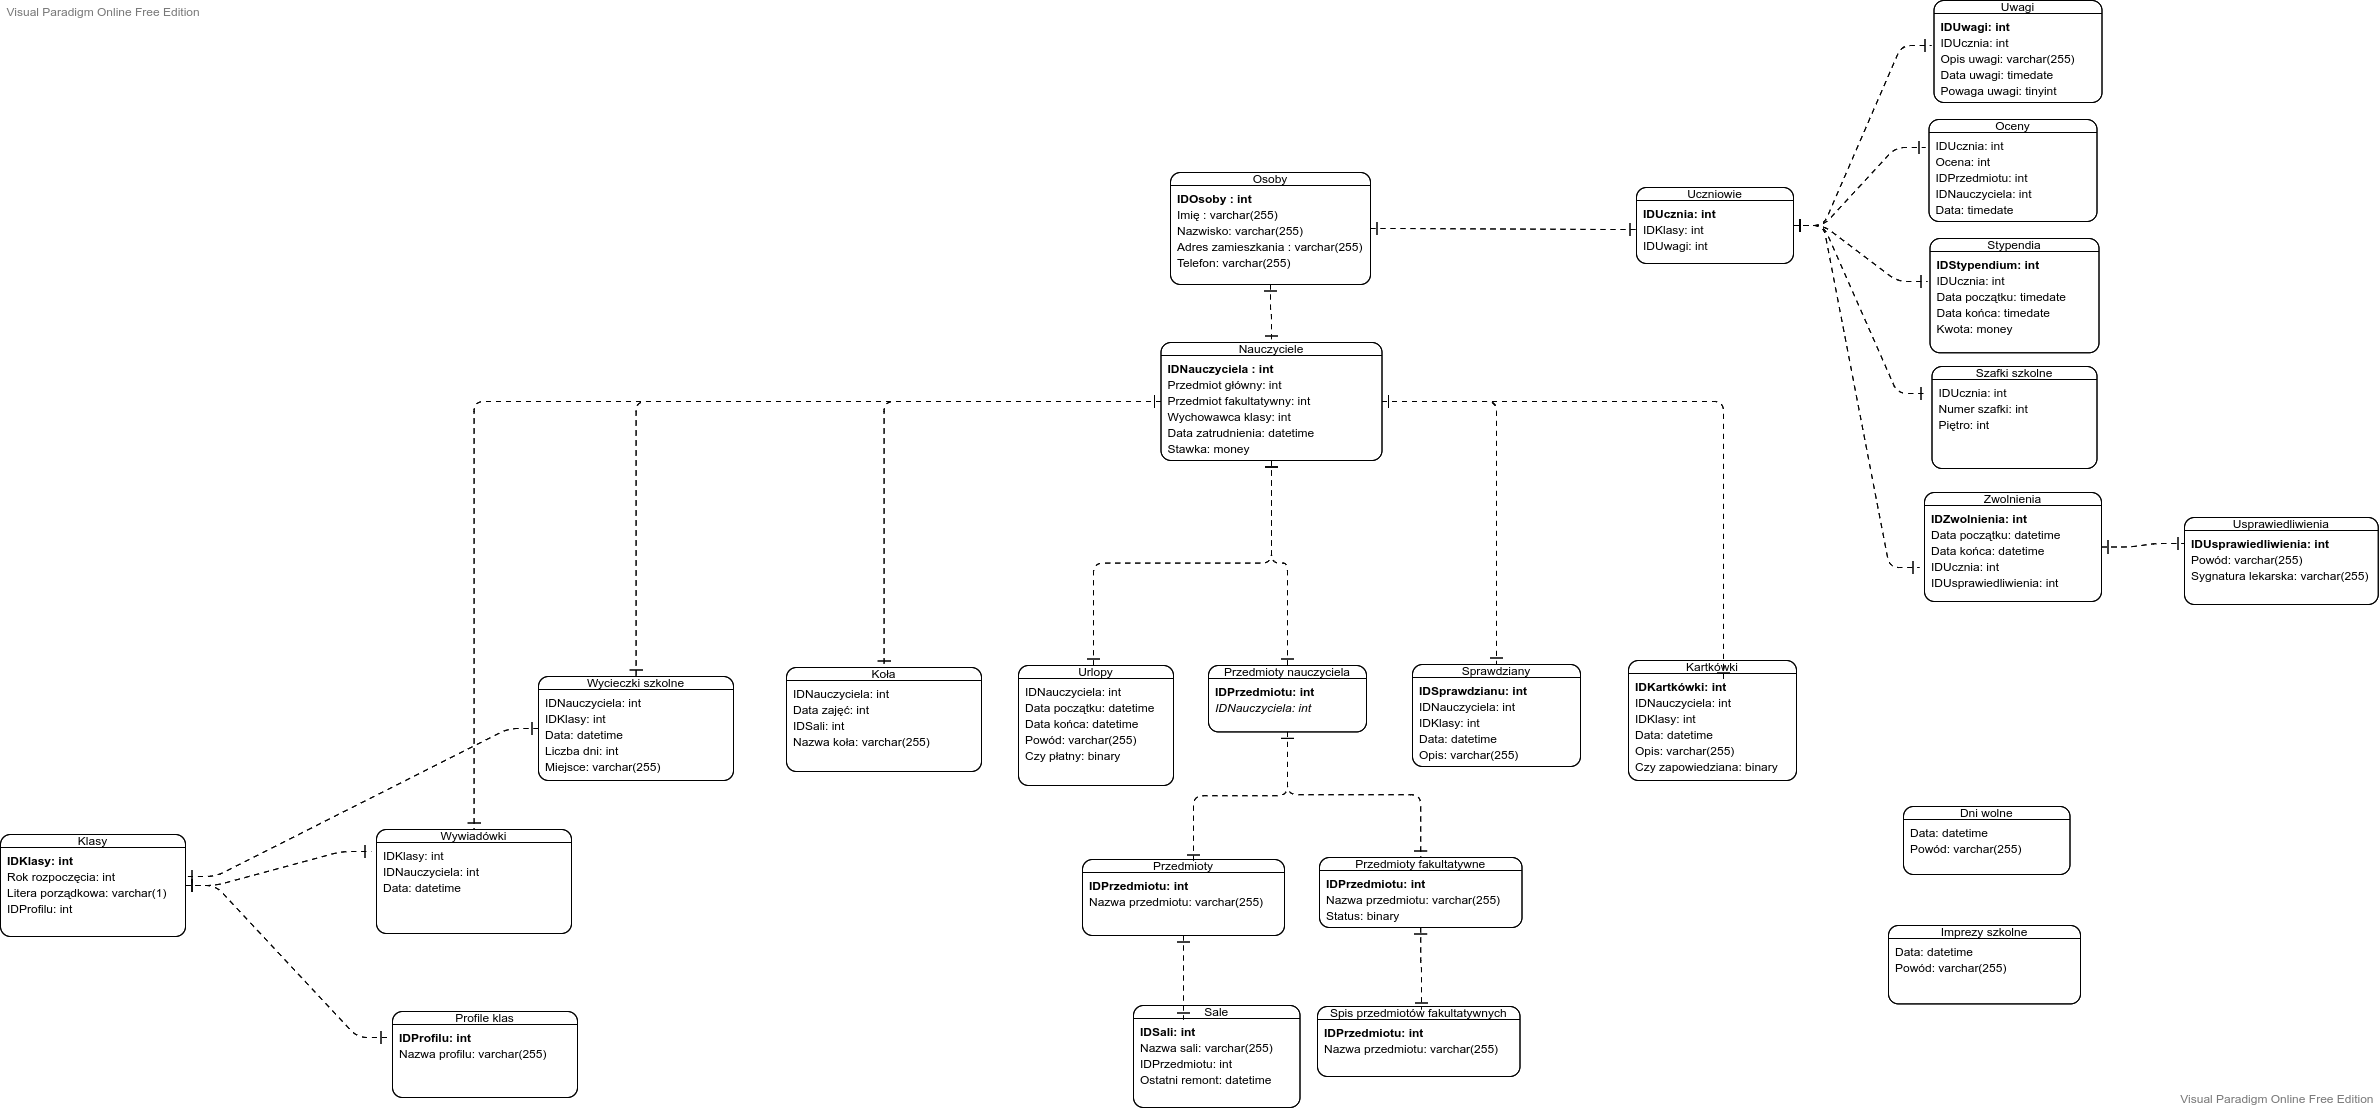
\includegraphics[width=\linewidth]{diagram_ER.png}
  \caption{Diagram ER}
  \label{Diagram ER}
\end{figure}

\subsection{Schemat bazy danych}

\newpage
\section{Dokumentacja technicza}

\subsection{Tabele}

Wymagania: 8 poprawnie zaprojektowanych tabel (na osobę).

\subsubsection{Osoby}
Jedna z podstawowych tabel bazy danych. Zawiera najistotniejsze dane o osobach uczestniczących do szkoły (nauczyciele i uczniowie) - ID, Imię, nazwisko, adres zamieszkania oraz telefon komórkowy.

\begin{minted}{sql}
--utworzenie tabeli
CREATE TABLE Osoby
(
	IDOsoby INT IDENTITY(1,1) PRIMARY KEY,
	Imię VARCHAR(255) NOT NULL,
	Nazwisko VARCHAR(255) NOT NULL,
	Telefon VARCHAR(255)
)

--wstawienie przykładowych osób
INSERT INTO [Osoby](Imię, Nazwisko, Telefon) VALUES
('Wojciech', 'Węgrzyn', '+48 723 147 680'),
('Konrad', 'Nowak', NULL),
('Jakub', 'Łukasiewicz', NULL),
('John',  'Grady', '+01 134 423 423'),
('Adrian', 'Antkiewicz', '+48 534 322'),
('Michał', 'Gem', '+18 332 03 42'),
('Piotr', 'Niemiec', '+12 890 43 54'), 
('Edward', 'Szczypka', '+12 345 54 23'), 
('Jadwiga', 'Kowal', NULL), 
('Iga', 'Świątek', NULL), 
('Andrzej', 'Gołota', '+48 543 134 543')

\end{minted}

\subsubsection{Nauczyciele}
 Jedna z podstawowych tabel bazy danych. Zawiera informacje o przedmiotach, jakie dany nauczyciel prowadzi (musi prowadzić jeden przedmiot główny, ale nie musi prowadzić fakultatywnego), jakiej klasy jest wychowawcą, kiedy został zatrudniony oraz ile zarabia miesięcznie.
 
 \begin{minted}{sql}
 --utworzenie tabeli
CREATE TABLE Nauczyciele
(
	IDNauczyciela INT REFERENCES Osoby(IDOsoby) 
	ON UPDATE CASCADE ON DELETE CASCADE PRIMARY KEY,
	WychowawcaKlasy INT REFERENCES Nauczyciele(IDNauczyciela),
	ON UPDATE CASCADE ON DELETE CASCADE PRIMARY KEY,
	DataZatrudnienia DATETIME,
	Stawka MONEY
)

--wstawianie nauczycieli
INSERT INTO [Nauczyciele]
(IDNauczyciela, WychowawcaKlasy, DataZatrudnienia, Stawka) 
VALUES
(4, NULL, GETDATE(), 5400),
(7, NULL, 2001-10-11, 15000),
(8, 1, 2013-08-01, 2300), 
(9, 2, 2020-01-01, 4500)

 \end{minted}
 
\subsubsection{Uczniowie}
Tabela przyporządkowująca danemu uczniowi klasę, do której chodzi, oraz uwagę, jaką dostał.
 
\begin{minted}{sql}
 --utworzenie tabeli
 CREATE TABLE Uczniowie
(
	IDUcznia INT REFERENCES Osoby(IDOsoby) ON UPDATE CASCADE ON DELETE CASCADE PRIMARY KEY,
	IDKlasy INT REFERENCES Klasy(IDKlasy) ON UPDATE CASCADE ON DELETE CASCADE NOT NULL,
	IDUwagi INT REFERENCES Uwagi(IDUwagi) ON UPDATE CASCADE ON DELETE CASCADE
)

--wstawienie uczniów
INSERT INTO [Uczniowie] (IDUcznia, IDKlasy, IDUwagi) VALUES
(1, 1, NULL),
(2, 1, NULL),
(3, 1, NULL),
(5, 2, 1),
(6, 2, 2), 
(10, 3, NULL), 
(11, 3, NULL)
\end{minted}
 
 \subsubsection{Oceny}
Tabela zawierająca informację o ocenach, które dostał dany uczeń - jej wartość, jaki nauczyciel ją wystawił i z jakiego przedmiotu oraz data wystawienia jej.
 
\begin{minted}{sql}
--utworzenie tabeli
CREATE TABLE Oceny
(
	IDUcznia INT REFERENCES Uczniowie(IDUcznia) 
	ON UPDATE CASCADE ON DELETE CASCADE NOT NULL,
	Ocena INT NOT NULL,
	IDPrzedmiotu INT REFERENCES Przedmioty(IDPrzedmiotu) 
	ON UPDATE CASCADE ON DELETE CASCADE NOT NULL,
	IDNauczyciela INT REFERENCES Nauczyciele(IDNauczyciela) 
	ON UPDATE CASCADE ON DELETE CASCADE NOT NULL,
	Data DATETIME
)

--wstawianie ocen
INSERT INTO [Oceny] (IDUcznia, Ocena, IDPrzedmiotu, IDNauczyciela, Data) VALUES
(1, 4, 1, 4, GETDATE()),
(1, 5, 1, 7, 2021-02-16),
(2, 2, 2, 7, 2021-02-16),
(3, 3, 2, 8, GETDATE()),
(10, 2, 3, 9, 2021-01-05)
\end{minted}

\subsubsection{Przedmioty}
 Prosta tabela będąca łącznikiem między nauczycielem a spisem przedmiotów. Zawiera tylko IDPrzedmiotu i IDNauczyciela (nauczyciel może uczyć tylko jeden przedmiot).
 
 \begin{minted}{sql}
--utworzenie tabeli
CREATE TABLE Przedmioty
(
	IDPrzedmiotu INT IDENTITY(1,1) NOT NULL,
	IDNauczyciela INT REFERENCES Nauczyciele(IDNauczyciela) 
	ON UPDATE CASCADE ON DELETE CASCADE NOT NULL,
)

--wstawianie przedmiotów
INSERT INTO [Przedmioty](IDNauczyciela) VALUES
(4),
(6), 
(4),
(6), 
(4),
(4) --TUTAJ JEST DO_SPRAWDZENIA
\end{minted}

\subsubsection{Przedmioty fakultatywne}
 Prosta tabela będąca łącznikiem między nauczycielem a spisem przedmiotów. Zawiera tylko IDPrzedmiotu i IDNauczyciela (nauczyciel może uczyć tylko jeden przedmiot fakulatywny, ale nie jest to obowiązkowe).
 
 \begin{minted}{sql}
--utworzenie tabeli
CREATE TABLE PrzedmiotyFakultatywne
(
	IDPrzedmiotuFakultatywnego INT IDENTITY(1,1),
	IDNauczyciela INT REFERENCES Nauczyciele(IDNauczyciela) 
	ON UPDATE CASCADE ON DELETE CASCADE NOT NULL,
)

--wstawianie przedmiotów fakultatywnych
INSERT INTO [PrzedmiotyFakultatywne](IDNauczyciela) VALUES
(4),
(6) --TUTAJ JEST DO_SPRAWDZENIA
\end{minted}

\subsubsection{Spis przedmiotów}
Prosta tabela przechowująca spis przedmiotów obowiązkowych z ich nazwami.

 \begin{minted}{sql}
--utworzenie tabeli
CREATE TABLE SpisPrzedmiotów
(
	IDPrzedmiotu INT PRIMARY KEY,
	NazwaPrzedmiotu VARCHAR(255)
)

--wstawianie przedmiotów
INSERT INTO [SpisPrzedmiotów](IDPrzedmiotu, NazwaPrzedmiotu) VALUES
(1, "Matematyka"),
(2, "Informatyka"),
(3, "Chemia"),
(4, "Język Polski"),
(5, "Biologia"),
(6, "Fizyka")
\end{minted}

\subsubsection{Spis przedmiotów fakultatywnych}
Prosta tabela przechowująca spis przedmiotów fakultatywnych z ich nazwami.

 \begin{minted}{sql}
--utworzenie tabeli
CREATE TABLE SpisPrzedmiotówFakultatywnych
(
	IDPrzedmiotuFakultatywnego INT PRIMARY KEY,
	NazwaPrzedmiotu VARCHAR(255)
)

--wstawianie przedmiotów fakultatywnych
INSERT INTO [SpisPrzedmiotów](IDPrzedmiotu, NazwaPrzedmiotu) VALUES
(7, "Etyka"),
(8, "Religia"),
\end{minted}

 \subsubsection{Sprawdziany}
Tabela zawierająca informację o sprawdzianach przeprowadzanych w szkole. Przechowuje informacje o nauczycielu, który przeprowadza ten sprawdzian, klasę, która go pisała, datę pisania oraz krótki opis zawierający np. opis materiału, jaki obejmował dany sprawdzian.
 
\begin{minted}{sql}
--utworzenie tabeli
CREATE TABLE Sprawdziany
(
	IDKartkówki INT IDENTITY(1,1) PRIMARY KEY,
	IDNauczyciela INT REFERENCES Nauczyciele(IDNauczyciela) 
	ON UPDATE CASCADE ON DELETE CASCADE NOT NULL,
	IDKlasy INT REFERENCES Klasy(IDKlasy) 
	ON UPDATE CASCADE ON DELETE CASCADE NOT NULL,
	Data DATETIME,
	Opis VARCHAR(255),
)

--wstawianie sprawdzianu
INSERT INTO [Sprawdziany](IDNauczycielam IDKlasy, Data, Opis) VALUES
(4, 1, 2021-10-12, "Rodziały 1-6"), 
(8, 2, 2020-01-10, "Cały zakres materiału"),
(9, 2, 2021-10-29, "Rodziały 7-9"), 
\end{minted}

 \subsubsection{Kartkówki}
Tabela zwierająca informację o kartkówkach przeprowadzanych przez danego nauczyciela dla danej klasy wraz z datą, opisem oraz informacją, czy była ona zapowiedziana czy nie.
 
\begin{minted}{sql}
--utworzenie tabeli
CREATE TABLE Kartkówki
(
	IDKartkówki INT IDENTITY(1,1) PRIMARY KEY,
	IDNauczyciela INT REFERENCES Nauczyciele(IDNauczyciela) 
	ON UPDATE CASCADE ON DELETE CASCADE NOT NULL,
	IDKlasy INT REFERENCES Klasy(IDKlasy) 
	ON UPDATE CASCADE ON DELETE CASCADE NOT NULL,
	Data DATETIME,
	Opis VARCHAR(255),
	CzyZapowiedziana BINARY
)

--wstawianie kartkówek
INSERT INTO [Kartkówki](IDNauczycielam IDKlasy, Data, Opis, CzyZapowiedziana) VALUES
(4, 1, GETDATE(), "Niezapowiedziana kartkówka z poprzedniej lekcji", NO), 
(8, 2, 2020-01-10, "Poprzednie 3 tematy", YES)
\end{minted}

 \subsubsection{Uwagi}
Tabela poświęcona uwagom ucznia. Zawiera IDUcznia, który dostał uwagę, krótki opis, datę oraz skalę powagi otrzymanej uwagi (w skali od 1-3, gdzie im większa liczba, tym poważniejsza uwaga).
 
\begin{minted}{sql}
--utworzenie tabeli
CREATE TABLE Uwagi
(
	IDUwagi INT IDENTITY(1,1) PRIMARY KEY,
	IDUcznia INT REFERENCES Uczniowie(IDUcznia) ON UPDATE CASCADE ON DELETE NOT NULL,
	OpisUwagi VARCHAR(255),
	DataUwagi DATETIME,
	PowagaUwagi TINYINT NOT NULL
)

--wstawianie kartkówek
INSERT INTO [Kartkówki](IDNauczycielam IDKlasy, Data, Opis, CzyZapowiedziana) VALUES
(4, 1, GETDATE(), "Niezapowiedziana kartkówka z poprzedniej lekcji", NO), 
(8, 2, 2020-01-10, "Poprzednie 3 tematy", YES)

--dodawanie uwag
INSERT INTO [Uwagi](IDUcznia, OpisUwagi, DataUwagi, PowagaUwagi) VALUES
(1, 'Bujał się na krześle', GETDATE(), 1), 
(1, 'Rozmawiał na lekcji', 2021-03-02, 1), 
(2, 'Ściągał na teście', GETDATE(), 2), 
(3, 'Pobił kolegę', 2021-04-11, 3)
\end{minted}

 \subsubsection{Stypendia}
Tabela poświęcona stypendium, które dostają najlepsi uczniowie. Zawiera IDUcznia, który je otrzymuje, datę rozpoczęcia i zakończenia wpłat oraz samą miesięczną kwotę stypendium.
 
\begin{minted}{sql}
--utworzenie tabeli
CREATE TABLE Stypendia
(
	IDStypendium INT IDENTITY(1,1) PRIMARY KEY,
	IDUcznia INT REFERENCES Uczniowie(IDUcznia) ON UPDATE CASCADE ON DELETE NOT NULL,
	DataPoczątku DATETIME,
	DataKońca DATETIME,
	Kwota MONEY
)

--przyznanie stypendium 
INSERT INTO [Stypendia](IDUcznia, DataPoczątku, DataKońca, Kwota) VALUES
(1, 2020-09-01, 2021-06-30, 500), 
(2, 2019-09-01, 2020-06-30, 1000),
(5, 2019-09-01, 2020-06-30, 200)
\end{minted}

 \subsubsection{Sale}
Informacja zawierająca informację o salach znajdujących się w szkole. Każda sala ma swoją własną nazwę oraz przyporządkowany do niej jeden przedmiot. Dodatkowo zawiera również datę ostatniego remontu sali.
 
\begin{minted}{sql}
--utworzenie tabeli
CREATE TABLE Sale
(
	IDSali INT IDENTITY(1,1) PRIMARY KEY,
	NazwaSali VARCHAR(255),
	IDPrzedmiotu INT REFERENCES Przedmioty(IDPrzedmiotu) ON UPDATE CASCADE ON DELETE CASCADE,
	OstatniRemont DATETIME
)

--dodawanie sal
INSERT INTO [Sale](NazwaSali, IDPrzedmiotu, OstatniRemont) VALUES
("23A", 1, 1993-03-04),
("1A", 2, 1895-02-13),
("1B, 3, GETDATE()),
("2", NULL, 2010-10-11),
("Świetlica", NULL, 2010-05-23)
\end{minted}

 \subsubsection{Klasy}
Tabela zawierająca klasy uczniów uczęszczających do szkoły. Tabela zawiera rok rozpoczęcia, literę porządkową (a, b itd.) oraz IDProfilu danej klasy.
 
\begin{minted}{sql}
--utworzenie tabeli
CREATE TABLE Klasy
(
	IDKlasy INT IDENTITY(1,1) PRIMARY KEY,
	RokRozpoczęcia INT NOT NULL,
	LiteraPorządkowa VARCHAR(1),
	IDProfilu INT REFERENCES ProfileKlas(IDProfilu) ON UPDATE CASCADE ON DELETE NOT NULL
)

--dodanie klasy
INSERT INTO [Klasy](RokRozpoczęcia, LiteraPorządkowa, IDProfilu) VALUES
(2019, 'A', 1),
(2019, 'B', 1),
(2018, 'A', 1),
(2018, 'B', 2),
(2017, NULL, 3)
\end{minted}


 \subsubsection{Profile klas}
Mała tabela zawierające IDProfilu oraz nazwę profilu klas w szkole.
 
\begin{minted}{sql}
--utworzenie tabeli
CREATE TABLE ProfileKlas
(
	IDProfilu INT IDENTITY(1,1) PRIMARY KEY,
	NazwaProfilu VARCHAR(255)
)

--dodanie profilów klas
INSERT INTO [ProfileKlas](NazwaProfilu) VALUES
('Mat-fiz'),
('Biol-chem'),
('Humanistyczny')
\end{minted}

 \subsubsection{Dni wolne}
Prosta tabela zawierająca datę oraz informację dotyczących dni wolnych podczas trwania roku szkolnego.
 
\begin{minted}{sql}
--utworzenie tabeli
CREATE TABLE DniWolne
(
	Data DATETIME,
	Powód VARCHAR(255)
)

--tworzenie dni wolnych
INSERT INTO [DniWolne](Data, Powód) VALUES
(2020-11-11, 'Dzień Niepodległości'),
(2020-12-23, 'Święta Bożego Narodzenia'),
(2020-12-24, 'Święta Bożego Narodzenia'),
(2020-12-25, 'Święta Bożego Narodzenia'),
(2020-12-26, 'Święta Bożego Narodzenia'),
(2020-12-31, 'Sylwester'),
(2021-01-01, 'Nowy Rok')
\end{minted}

 \subsubsection{Wywiadówki}
Tabela przechowująca dane o wywiadówkach przeprowadzanych w trakcie roku szkolnego, zawierająca jaki nauczyciel dla jakiej klasy przeprowadzał daną wywiadówkę wraz z datą.
 
\begin{minted}{sql}
--utworzenie tabeli
CREATE TABLE Wywiadówki
(
	IDKlasy INT REFERENCES Klasy(IDKlasy) ON UPDATE CASCADE ON DELETE NOT NULL,
	IDNauczyciela INT REFERENCES Nauczyciele(IDNauczyciela) ON UPDATE CASCADE ON DELETE,
	Data DATETIME
)

--dodanie wywiadówki
INSERT INTO [Wywiadówki](IDKlasy, IDNauczyciela, DATA) VALUES
(1, 4, 2020-10-12),
(2, 8, 2020-12-12),
(3, 4, 2021-01-20),
(4, 9, 2021-02-10)
\end{minted}

 \subsubsection{Koła}
Tabela przechowująca informacje odnośnie kół zainteresowań w szkole. Zawiera informacje o nauczycielu opiekującym się kołem, dacie odbywania się zajęć, salę, w której się odbywają spotkania oraz nazwę koła.
 
\begin{minted}{sql}
--utworzenie tabeli
CREATE TABLE Koła
(
	IDNauczyciela INT REFERENCES Nauczyciele(IDNauczyciela) ON UPDATE CASCADE ON DELETE NOT NULL,
	DataZajęć INT NOT NULL,
	IDSali INT REFERENCES Sale(IDSali) ON UPDATE CASCADE ON DELETE NOT NULL,
	NazwaKoła VARCHAR(255) NOT NULL
)

--wstawianie sal
INSERT INTO [Koła](IDNauczyciela, DataZajęć, IDSali, NazwaKoła) VALUES
(4, 2021-02-10, 1, 'Koło Informatyczne'),
(4, 2021-02-12, 1, 'Koło Matematyczne')
\end{minted}

 \subsubsection{Wycieczki szkolne}
 Tabela przechowująca informacje odnośnie wycieczek szkolnych, które odbyły się w trakcie trwania roku szkolnego. Każda wycieczka szkolna ma nauczyciela, który był podczas jej trwania opiekunem, klasę, jaka pojechała na tę wycieczkę, datę odbycia oraz czas trwania w dniach oraz miejsce, do którego się udali.
\begin{minted}{sql}
--utworzenie tabeli
CREATE TABLE WycieczkiSzkolne
(
	IDNauczyciela INT REFERENCES Nauczyciele(IDNauczyciela) ON UPDATE CASCADE ON DELETE NOT NULL,
	IDKlasy INT REFERENCES Klasy(IDKlasy) ON UPDATE CASCADE ON DELETE NOT NULL,
	Data DATETIME,
	LiczbaDni INT,
	Miejsce VARCHAR(255)
)

--wstawianie wycieczek
INSERT INTO [WycieczkiSzkolne](IDNauczyciela, IDKlasy, Data, LiczbaDni, Miejsce) VALUES
(4, 1, 2020-10-10, 5, 'Zagrzeb'),
(4, 2, 2020-12-01, 2, 'Kraków'),
(8, 1, 2021-01-02, 1, 'Warszawa'),
(8, 3, 2020-10-20, 4, 'Berlin'),
(9, 2, 2019-10-12, 3, 'Lwów'),
(9, 1, 2019-12-30, 1, 'Zakopane')
\end{minted}

 \subsubsection{Szafki szkolne}
 Prosta tabela przechowująca informację o szafce szkolnej danego ucznia, wraz z jej numerem oraz piętrem, na którym się znajduje.

\begin{minted}{sql}
--utworzenie tabeli
CREATE TABLE SzafkiSzkolne
(
	IDUcznia INT REFERENCES Uczniowie(IDUcznia) ON UPDATE CASCADE ON DELETE NOT NULL,
	NumerSzafki INT PRIMARY KEY,
	Piętro INT
)

--wstawienie szafki
INSERT INTO [SzafkiSzkolne](IDUcznia, NumerSzafki, Piętro) VALUES
(1, 10, 0),
(2, 11, 0),
(3, 12, 0),
(10, 33, 1),
(5, 1, 1),
(6, 2, 1),
(11, 3, 2)
\end{minted}

 \subsubsection{Imprezy szkolne}
Prosta tabela przechowująca informacja odnośnie imprez szkolnych, które odbyły się w trakcie roku wraz z datą oraz przyczyną zorganizowania.

\begin{minted}{sql}
--utworzenie tabeli
CREATE TABLE ImprezySzkolne
(
	Data DATETIME,
	Powód VARCHAR(255)
)

--wstawianie imprez
INSERT VALUES [ImprezySzkolne](Data, Powód) VALUES
(2021-01-02, "Nowy Rok"),
(2020-06-15, "Zakończenie roku szkolnego"),
(2020-10-10, "Andrzejki"),
(2021-02-14, "Walentynki"),
(GETDATE(), "Spontaniczna impreza")
\end{minted}

 \subsubsection{Urlopy}
Tabela zawierająca informacje odnośnie urlopów nauczycieli wraz z datami rozpoczęcia oraz zakończenia danego urlopy z podanym powodem oraz informacją, czy był płatny, czy nie.

\begin{minted}{sql}
--utworzenie tabeli
CREATE TABLE Urlopy
(
	IDNauczyciela INT REFERENCES Nauczyciele(IDNauczyciela) ON UPDATE CASCADE ON DELETE NOT NULL,
	DataPoczątku DATETIME NOT NULL,
	DataKońca DATETIME,
	Powód VARCHAR(255),
	CzyPłatny BINARY NOT NULL,
)

--wstawianie urlopów
INSERT INTO [Urlopy](IDNauczyciela, DataPoczątku, DataKońca, Powód, CzyPłatny) VALUES
(4, 2021-01-01, 2021-01-02, "Kac noworoczny", NO),
(4, 2021-04-01, 2021-04-30, "Złamana noga", YES),
(8, 2020-10-01, 2020-12-30, "Problemy rodzinne", NO)
\end{minted}

 \subsubsection{Zwolnienia}
Tabela przechowująca informacje odnośnie zwolnień ucznia wraz z datami początku i końca zwolnienia, z odnośnikiem do ucznia oraz usprawiedliwienia.

\begin{minted}{sql}
--utworzenie tabeli
CREATE TABLE Zwolnienia
(
	IDZwolenienia INT IDENTITY(1,1) PRIMARY KEY,
	DataPoczątku DATETIME,
	DataKońca DATETIME,
	IDUcznia INT REFERENCES Uczniowie(IDUcznia)ON UPDATE CASCADE ON DELETE CASCADE NOT NULL,
	IDUsprawiedliwienia INT REFERENCES Usprawiedliwienia(IDUsprawiedliwienia)ON UPDATE CASCADE ON DELETE CASCADE
)

--wstawianie zwolnień
INSERT INTO [Zwolnienia](DataPoczątku, DataKońca, IDUcznia, IDUsprawiedliwenia) VALUES
(2020-10-10, 2020-10-11, 1, NULL),
(2021-03-02, 2021-03-02, 2, 1)
\end{minted}

 \subsubsection{Usprawiedliwienia}
Prosta table zawierająca informacje odnośnie usprawiedliwienia dla zwolnienia ucznia. Zawiera ona IDUsprawiedliwienia, powód oraz sygnaturę lekarską potwierdzającą to usprawiedliwienie.

\begin{minted}{sql}
--utworzenie tabeli
CREATE TABLE Usprawiedliwienia
(
	IDUsprawiedliwienia INT IDENTITY(1, 1) PRIMARY KEY,
	Powód VARCHAR(255),
	SygnaturaLekarska VARCHAR(255)
)

--wstawianie usprawiedliwienia 
INSERT INTO [Usprawiedliwienia](Powód, SygnaturaLekarska) VALUES
("Złamana noga", "L/13/202"),
("Osłabienie", "L/13/201"), 
("Biegunka", "L/01/01")
\end{minted}

\subsection{Widoki oraz funkcje}

Wymagania: 10 widoków lub funkcji.

\subsection{Procedury i wyzwalacze}

Wymagania: baza danych powinna być odpowiednio oprogramowana z wykorzystaniem procedur składowanych i wyzwalaczy (co najmniej po 5 procedur i po 5 wyzwalaczy).





\end{document}